\documentclass{article}
\usepackage[T1]{fontenc}
\usepackage{lmodern}
\usepackage{graphicx}
\usepackage{amsmath,amssymb}
\usepackage[a4paper,margin=2cm]{geometry}
\usepackage[absolute,overlay]{textpos}
\setlength{\TPHorizModule}{1mm}
\setlength{\TPVertModule}{1mm}
\usepackage[indonesian]{babel}
\usepackage{hyperref}
\setlength{\emergencystretch}{2em}
% unit: Halaman 25

\begin{document}

% === Halaman 25 (llm) ===

\section*{Public-Key Encryption by RSA Algorithm}

\subsection*{Objective}
The purpose of this page is to demonstrate step by step how a public-key encryption system works. We use the RSA algorithm (named after the inventors Rivest, Shamir, Adleman) with very small primes. The basic functions are implemented in JavaScript and can be viewed in the source.

\textbf{Note:} This page is only for explaining the mechanism. In practice more advanced algorithms and much larger primes are used!

\subsection*{Overview}
Working with a public-key encryption system has mainly three phases:

\begin{enumerate}
    \item \textbf{Key Generation:} Whoever wants to receive secret messages creates a public key (which is published) and a private key (kept secret). The keys are generated in a way that conceals their construction and makes it 'difficult' to find the private key by only knowing the public key.
    \item \textbf{Encryption:} A secret message to any person can be encrypted by his/her public key (that could be officially listed like phone numbers).
    \item \textbf{Decryption:} Only the person being addressed can easily decrypt the secret message using the private key.
\end{enumerate}

\subsection*{RSA Key Generation}
From two selected primes the computer will generate the public and the private key:

Pick 2 (different) primes: $p = 7$ $\quad q = 11$ \vspace{10mm}

\vspace{35.64mm}

\begin{align*}
    n &= 77 && (n = p.q) \\
    \varphi &= 60 && (\varphi = \varphi(n) = (p-1).(q-1); \text{ needed to determine e and d}) \\
    e &= 7 && (\text{arbitrary, but less than n and relatively prime to } \varphi)
\end{align*}

% deskripsi: Screenshot area input interaktif untuk pemilihan bilangan prima p dan q serta tombol Generate keys
% bbox normalisasi: [0.1500, 0.7800, 0.3900, 0.8400]
\begin{textblock*}{50.40mm}(31.50mm,231.66mm)
\noindent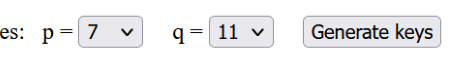
\includegraphics[width=50.40mm,height=17.82mm]{../../images/llm/page_025_img_01.png}%
\end{textblock*}

% deskripsi: Screenshot area output kalkulasi nilai n, phi, dan e dalam proses pembuatan kunci RSA
% bbox normalisasi: [0.3400, 0.8400, 0.7100, 0.9600]
\begin{textblock*}{77.70mm}(71.40mm,249.48mm)
\noindent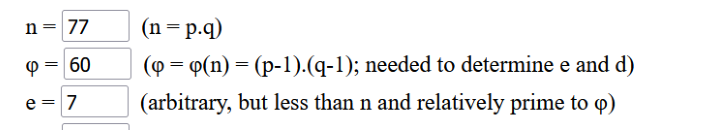
\includegraphics[width=77.70mm,height=35.64mm]{../../images/llm/page_025_img_02.png}%
\end{textblock*}

\end{document}
